\documentclass[11pt]{amsart}
\usepackage[margin=1in]{geometry}                % See geometry.pdf to learn the layout options. There are lots.
\geometry{letterpaper}                   % ... or a4paper or a5paper or ... 
%\geometry{landscape}                % Activate for for rotated page geometry
\usepackage[parfill]{parskip}    % Activate to begin paragraphs with an empty line rather than an indent
\usepackage{graphicx, tikz, enumerate}
\usetikzlibrary{calc}
\usepackage{amssymb}
\usepackage[normalem]{ulem}
\usepackage{epstopdf}
\DeclareGraphicsRule{.tif}{png}{.png}{`convert #1 `dirname #1`/`basename #1 .tif`.png}

\title{Brief Article}
\author{The Author}
%\date{}                                           % Activate to display a given date or no date


\usepackage{hyperref}

%\newcommand{\deg}{\mathrm{deg}}

\newcommand{\bv}[1]{\ensuremath{\mathbf{#1}}}
\newcommand{\be}{\begin{enumerate}}
\newcommand{\ee}{\end{enumerate}}

\begin{document}
\begin{center}
\begin{Large} Math F307 \hfill Spring 2017

Homework Exercises 
\end{Large}
\end{center}
%\maketitle
%\section{}
%\subsection{}

\subsection*{Instructions for writing up homework}
\begin{itemize}
\item Although you are encouraged to work with your classmates on the homework assignments, you must write up the solutions individually.
\item Read the section!
 \item Use pen or non-smeary pencil. Do not have little scritchies on the side. 
 \item Staple your homework. 
 \item Write legibly, and leave lots of whitespace. Make sure your writing is dark enough to be readable. If this is problematic for you, consider typing your homework.
 \item Answer the question in complete sentences, where appropriate.
\item {\bf Write the \fbox{problem statements} as well as the answers. } This is not optional. \underline{Points will be deducted if you do not do this}.
\item Have headings indicating the section.
\item {\bf In the upper right hand corner of your top page,} write your name (first and last) on your assignment, along with the course number (Math 307) and which assignment it is.
\item {\bf You are expected to ask questions in class about the homework problems!}
\end{itemize}

\section*{Homework Set 7}

{\bf DUE Friday, March 12 \fbox{at the beginning of class}. No late homework, especially this week.}
You should {\bf read} each section!

\subsection*{Section 6.3}

Think about, but do not turn in: 1, 3c, 7, 9, 14

To turn in:  2 (provide a labelling proving the isomorphism), 8, 11a

\subsection*{Section 6.4} 

(Also Worksheet on Pr\"{u}fer Codes, not in your textbook)

Think about, but do not turn in: 1, 3, 5, 7

To turn in: 6, 8, 10, 12

Turn in these additional:

\be
\item Draw a tree with Pr\"ufer code $(5,2,1,4,4,1,6,1,1)$, with no crossing edges. Show some work.
\item Find the Pr\"{u}fer code of the following tree. Show some work.

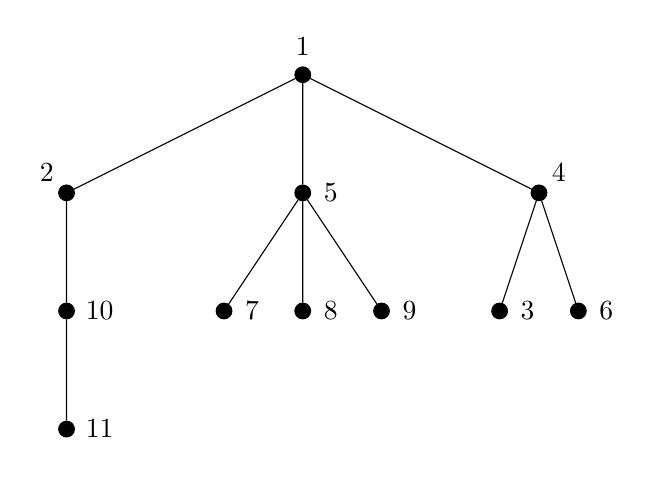
\begin{tikzpicture}[scale = 1,every node/.style={circle,draw, fill= black, inner sep = 2pt},level 1/.style={sibling distance=30mm},level 2/.style={sibling distance=10mm}
]
\node[label = above:1] {}
child { node[label = above left:2] {} child { node[label = right:10] {} child { node[label = right:11] {} }}}
child { node[label = right:5] {} 
child { node[label = right:7] {} }
child { node[label = right:8] {} }
child { node[label = right:9] {} }
}
child { node[label = above right:4] {} 
child { node[label = right:3] {} }
child { node[label = right:6] {} }};

\end{tikzpicture}
\ee

\subsection*{Section 6.5} 

Think about, but do not turn in: 3, 7, 9, 10, 13

To turn in:  2, 4, 8

\subsection*{Section 4.6}

To Turn in: \# 8


\end{document}